\subsection{Nonlinear elastic axisymmetric triaxial compression}
\label{subsec:Me6}

\subsubsection{Definition}
\label{subsubsec:Me6_def}

Triaxial short-term compression under axisymmetric conditions is carried out to verify the nonlinear elastic isotropic material model (modified Lubby1 approach). The loading in principal axes includes a radial pressure as well as an axial displacement, and is realized in two steps. It is resulting in a homogeneous stress-strain state. 

\subsubsection{Solution}
\label{subsubsec:Me6_sol}

For the calculation, the cross-section of a cylindrical sample with a radius of $30\,\mbox{mm}$ and a height of $120\,\mbox{mm}$ is studied. Details of the model (geometry, mesh, boundary conditions) according to K.-H. Lux and F. Werunsky (unpublished report, 2008) are presented in Fig.~\ref{Me_triax_model_lubby1}.
\begin{figure}[!htb]
\begin{center}
\includegraphics[width=0.2\textwidth]{PART_II/M/svv_model.eps}
\hspace*{10.0ex}
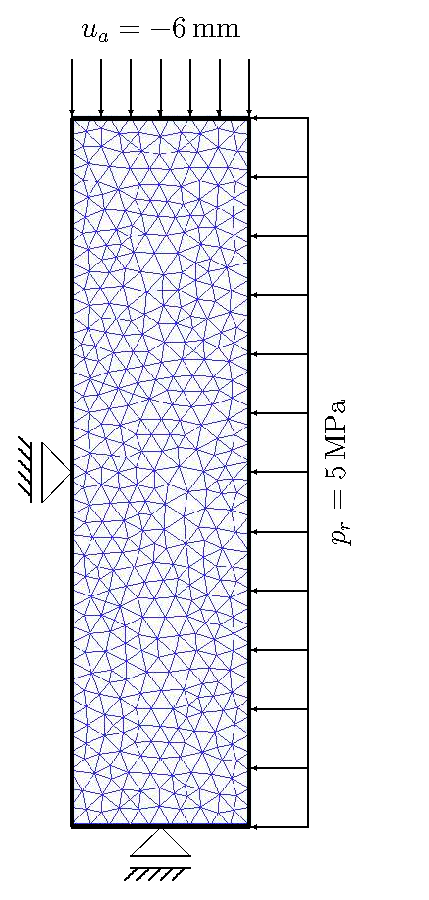
\includegraphics[width=0.25\textwidth]{PART_II/M/svv_mesh.eps}
\end{center}
\caption{Triaxial compression of a cylindrical sample. Axisymmetric model. Left: Geometry. Right: Finite element grid and boundary conditions} 
\label{Me_triax_model_lubby1}
\end{figure}

Initial conditions do not have to be given for the problem under consideration. As the bottom edge is fixed in vertical direction, the left-hand edge is fixed in horizontal direction for symmetry reasons (axis of rotation). On the right-hand edge initially a radial casing pressure of $5\,\mbox{MPa}$ is applied within 20~seconds with a constant stress rate. While keeping constant this radial pressure, a subsequent stroke-driven axial compressive loading is applied within the following 1440~seconds with a constant strain rate. The maximum axial displacement is $6\,\mbox{mm}$ which corresponds to a $5\,\%$ reduction of the sample's height (for the complex loading history cf. Fig.~\ref{Me_triax_loadhist_lubby1}).
\begin{figure}[!htb]
\begin{center}
\includegraphics[width=0.75\textwidth]{PART_II/M/svv_loadhistory.eps}
\end{center}
\caption{Triaxial compression of a cylindrical sample. Loading history for short-term experiments. Radial casing pressure (stress rate $\dot{p}{}_r=0.25$\,MPa$\cdot$s$^{-1}$) with subsequent axial displacement (strain rate $\dot{\varepsilon}{}_a=3.47\times 10^{-5}$\,s$^{-1}$)} 
\label{Me_triax_loadhist_lubby1}
\end{figure}
 
The material parameters referring to the modified Lubby1 relation~(\ref{Me_lubby1_ev}) are summarized in Tab.~\ref{Me_matpar_lubby1}. Within this context, the initial Young's modulus and the Poisson's ratio are close to values known for rock salt.
 
%\vskip 3.0ex
 
\begin{table}[!htb]
\centering
\caption{Material parameters}
\label{Me_matpar_lubby1}
\begin{tabular}{llll}
\toprule
Symbol & Parameter & Value & Unit \\
\midrule
$E_0$ & Initial Young's modulus          & $21.4$  & GPa \\
$\nu$ & Poisson's ratio                  & $0.335$ & --  \\
$a$   & Factor in (\ref{Me_lubby1_ev})   & $2750$  & --  \\
$n$   & Exponent in (\ref{Me_lubby1_ev}) & $1.0$   & --  \\
\bottomrule
\end{tabular}
\end{table}

\subsubsection{Results}
\label{subsubsec:Me6_res}

The representation of the axial stress vs. the axial strain in Fig.~\ref{Me_triax_res_lubby1} shows on exemplarily chosen material parameters the noticeable difference between the linear (Hooke's model) and the nonlinear (modified Lubby1 model) elastic models even at small strains. Within the contect of the studied case, the stress response will be overestimated by a multiple using the linear Hooke's law. 

%\clearpage

\begin{figure}[!htb]
\begin{center}
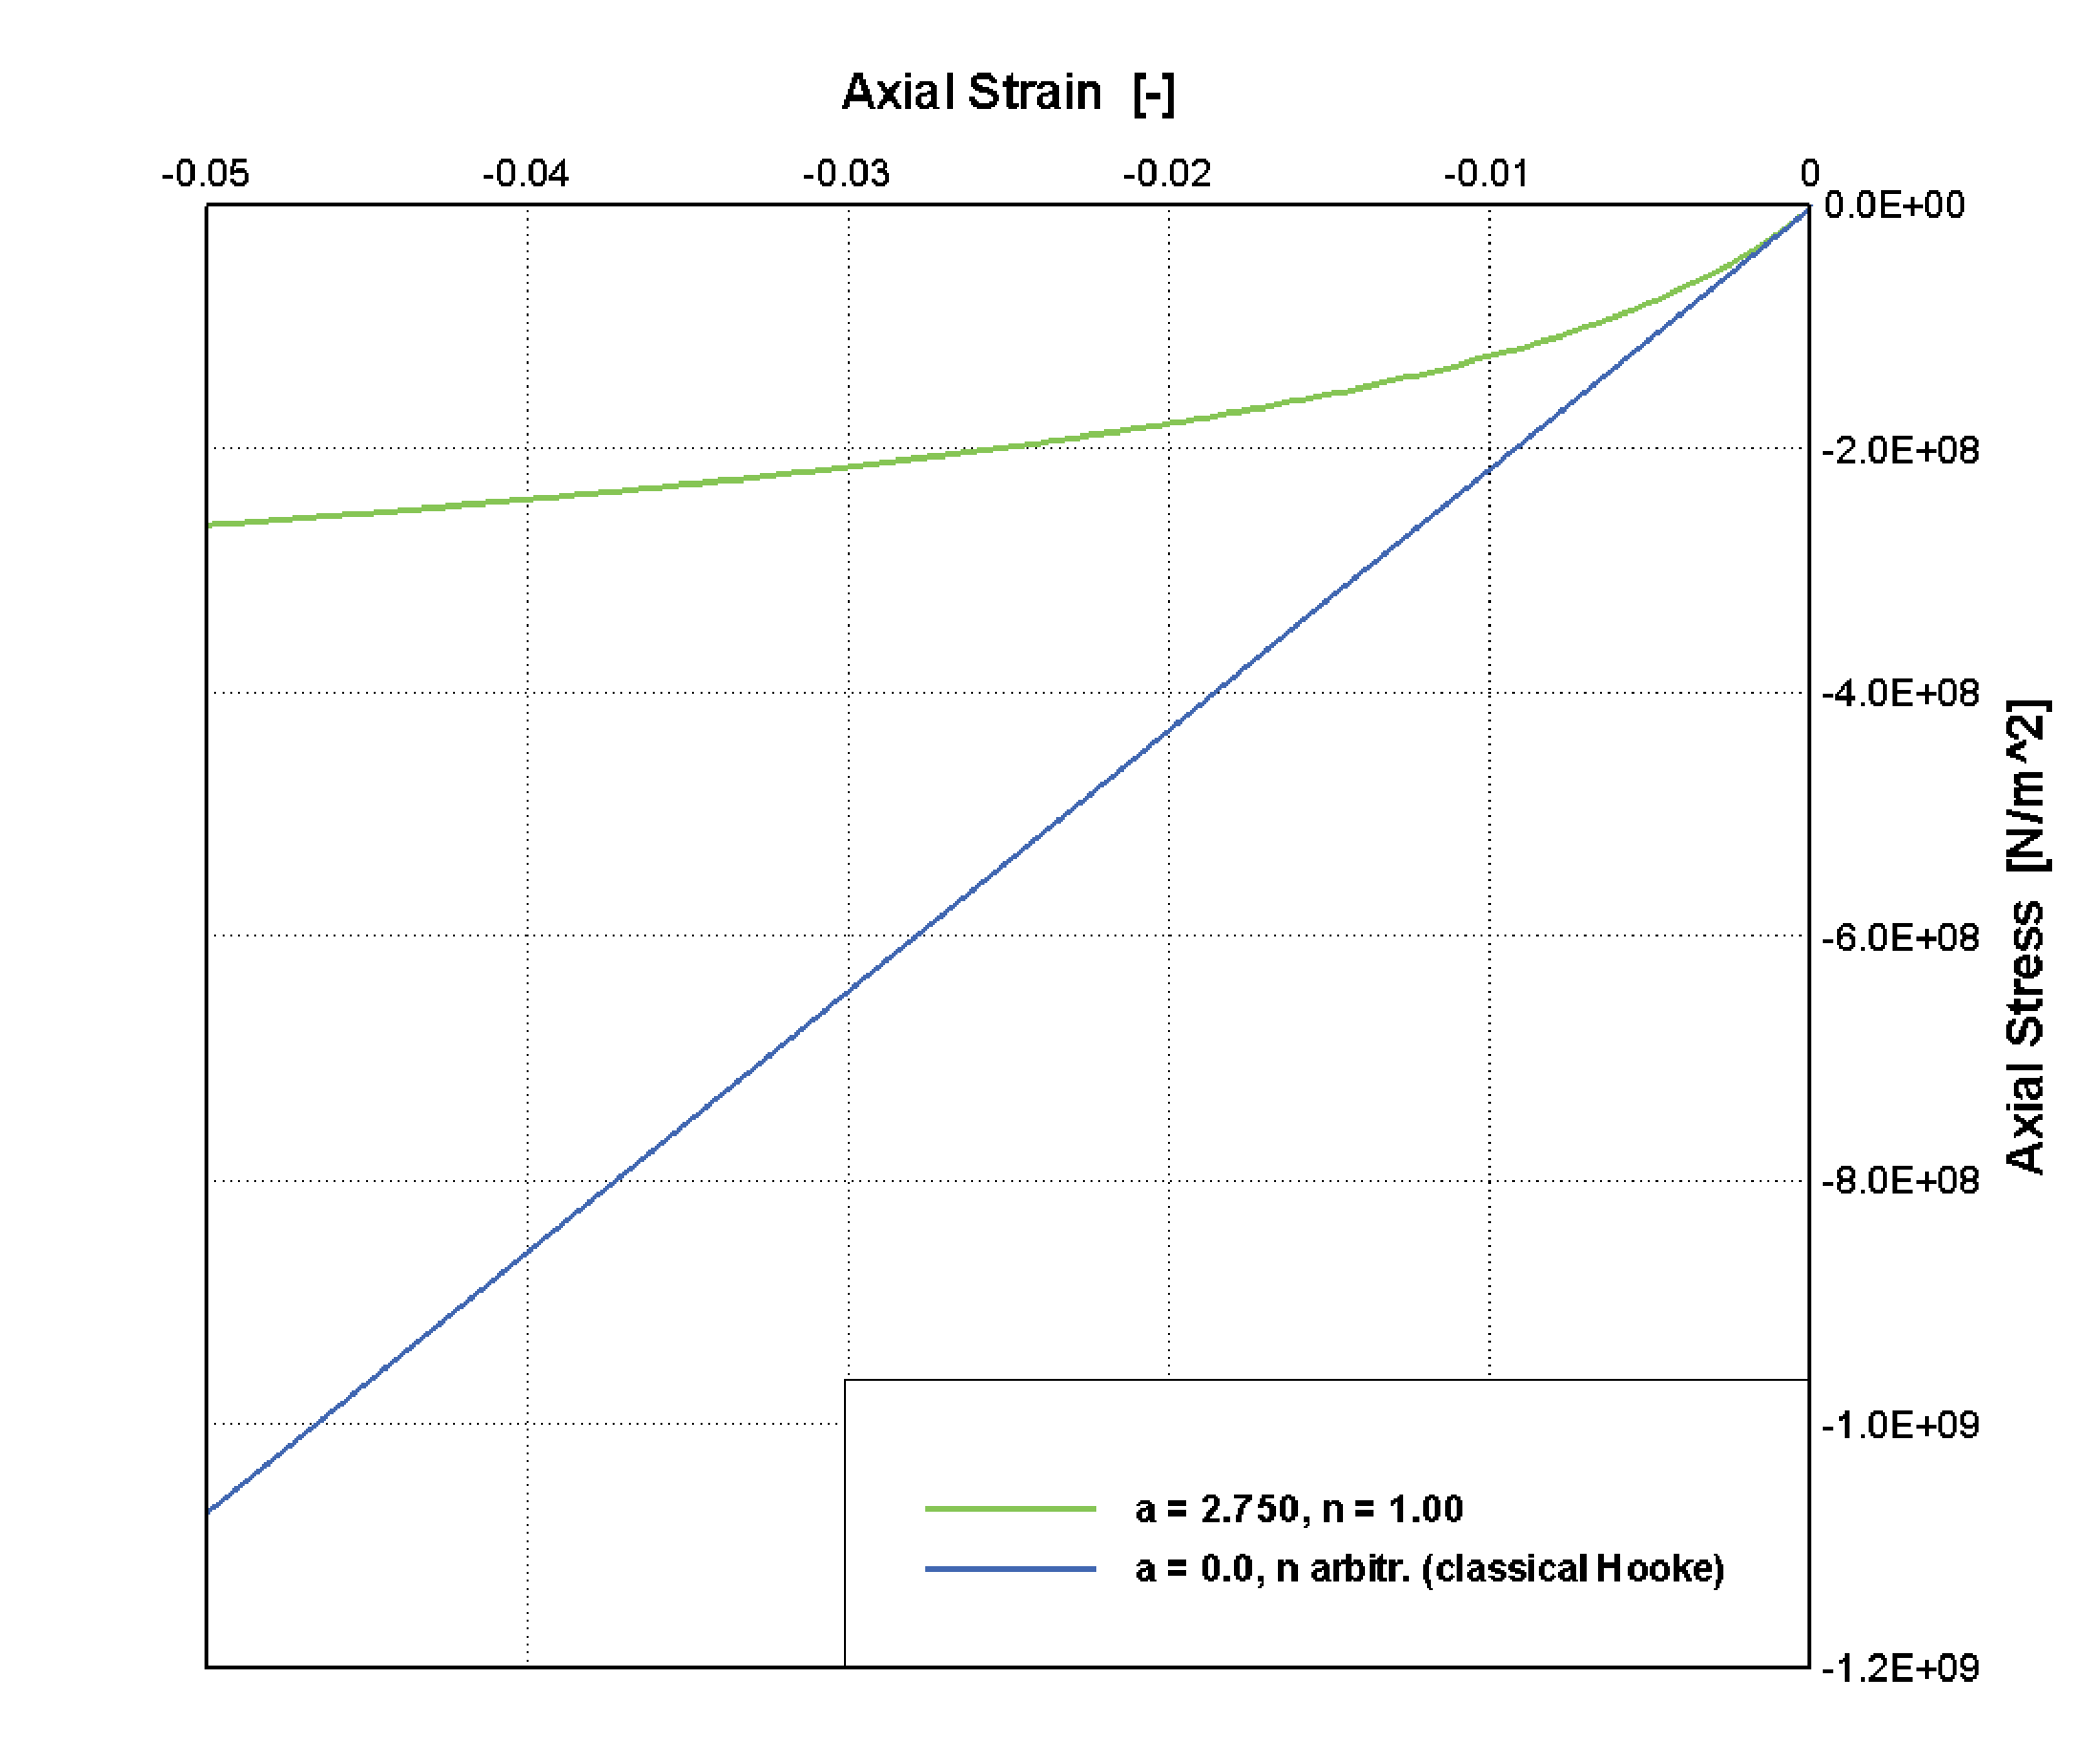
\includegraphics[width=0.75\textwidth]{PART_II/M/svv_e_stress_strain_hooke_lubby1m.eps}
\end{center}
\caption{Triaxial compression of a cylindrical sample. Stress-strain curves regarding the axial load response. Comparison of linear elastic (Hooke) and nonlinear elastic (modified Lubby1~(\ref{Me_lubby1_ev})) material models} 
\label{Me_triax_res_lubby1}
\end{figure}

